\begin{center}
\begin{tikzpicture}
	\node[anchor=south west,inner sep=0] (image)  at (0,0) {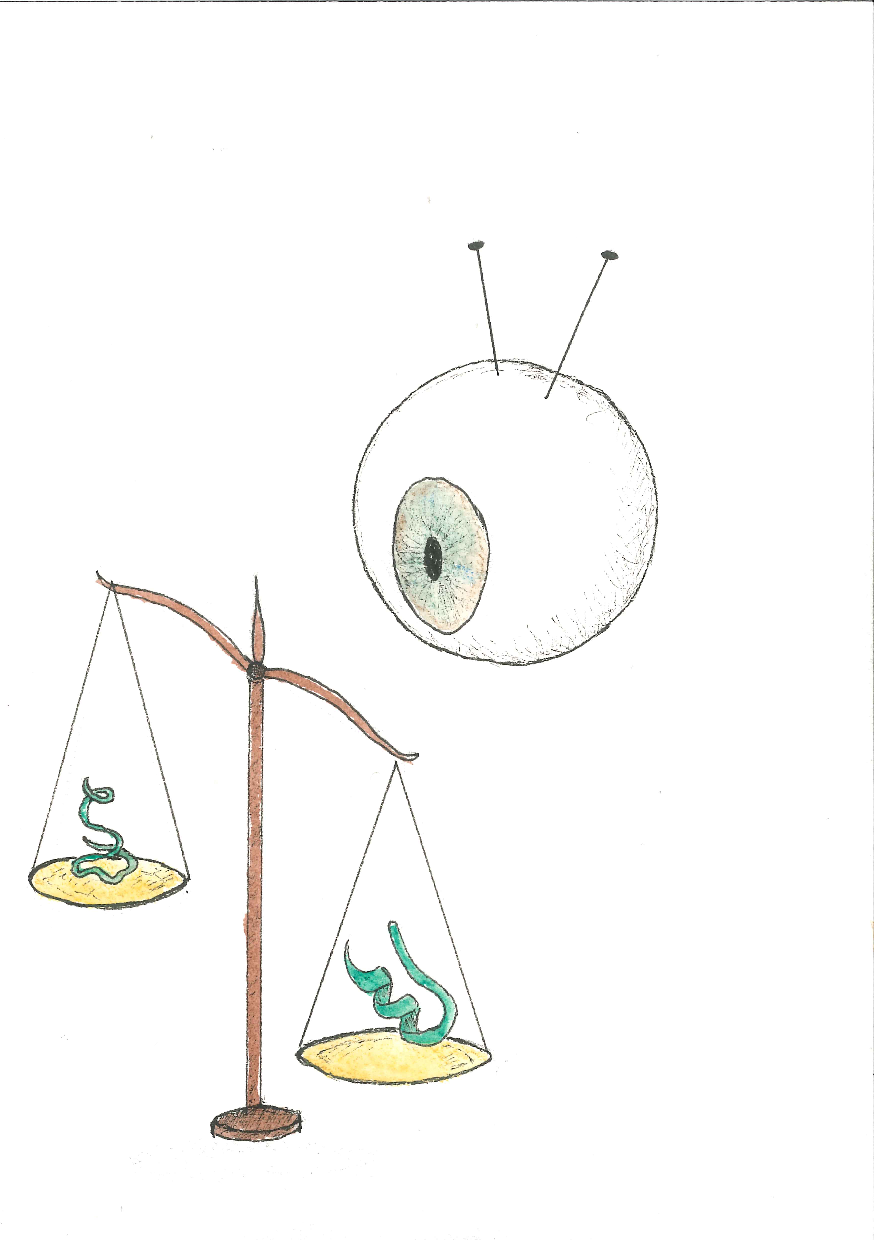
\includegraphics[trim={2mm, 2mm, 2mm, 2mm}, width=0.995\pagewidth]{scans/panel-6.pdf}};
    \begin{scope}[x={(current page.south east)},y={(current page.north west)}]
		\if\helplines1
			\draw[help lines,xstep=.1,ystep=.1] (0,0) grid (\N, \N);
		\else
			\path[help lines,xstep=.1,ystep=.1] (0,0) grid (\N, \N);
		\fi
		\node(title) at (0.5, 0.9) {\Huge {\color{Maroon}IV} - ProQ4};
		\node[text width=0.4\pagewidth, align=justify, anchor=north west](a) at (0.06, 0.85) {\english{We followed the same minimalistic philosophy for training a program to asess the quality of models. ProQ4 is another lightweight, fast, and easy to use program to evaluate the quality of models.}};
		
		\node[text width=0.4\pagewidth, align=left, anchor=north west, below=7mm of a]  {\english{\doindent The key insight that fuels\\ its quality is that we focused
		\\ the training in comparing \\models, rather than just\\ classifying them as “good”\\ or “bad”.}};
		
		\node[text width=0.4\pagewidth, align=justify, anchor=north ](b) at (0.759, 0.44) {\spanish{Aplicamos la misma filosofía para entrenar un programa que estime la calidad de modelos de proteínas. ProQ4 es otro programa rápido, ligero y fácil de usar para evaluar la calidad de modelos de proteínas.}};
		
		%\node[text width=0.4\pagewidth, align=justify, anchor=north west, below=7mm of b]{\spanish{\doindent en lugar de simplemente clasificarlos como “buenos” o “malos”.}};
		\node[text width=0.4\pagewidth, align=justify, anchor=north west, below=7mm of b]{\spanish{\doindent La idea clave detrás de la calidad de los resultados es que concentramos el entrenamiento en comparar modelos, en lugar de simplemente clasificarlos como <<buenos>> o <<malos>>.}};  
    \end{scope}

\end{tikzpicture}
\end{center}
